
\documentclass[12pt]{article}
\usepackage[utf8]{inputenc}
\usepackage{amsmath, amssymb}
\usepackage{graphicx}
\usepackage{natbib}
\usepackage{geometry}
\usepackage{hyperref}
\geometry{margin=1in}

\title{Report on Fast Mesh-to-Mesh Remaps Using Hash Algorithms}
\author{Kaixiang Zou}
\date{April 2025}

\begin{document}

\maketitle

\begin{abstract}
This report presents a detailed study on fast mesh-to-mesh remapping algorithms based on hash structures. The remapping process is crucial in computational physics simulations, where data must be transferred between different spatial discretizations efficiently and accurately.

We investigate several variants of hash-based methods, including hierarchical hash tables and memory-optimized strategies, as alternatives to traditional kD-tree-based approaches. The proposed techniques significantly reduce memory operations and enable rapid remapping for large-scale meshes.

Experimental evaluations on 2-D mesh data demonstrate that the hash-based methods achieve up to two orders of magnitude speedup over classical techniques, with competitive accuracy. We further analyze their performance across serial CPU, multi-core CPU (OpenMP), and GPU (OpenCL) implementations, confirming their scalability and suitability for high-performance computing environments.


\end{abstract}

\tableofcontents

\section{Introduction}

In recent years, Graphics Processing Units (GPUs) have become the backbone of modern high-performance computing (HPC) and artificial intelligence (AI) workloads. Their massive parallelism and high memory bandwidth make them especially well-suited for accelerating tasks such as training large language models (LLMs), image processing, and scientific simulations. With the exponential growth of LLMs, such as GPT-3 and Llama-2, the demand for more powerful and efficient GPU architectures continues to rise.

To meet this demand, Nvidia has continuously released new GPU architectures every two years, with each generation introducing improvements in computational performance, memory hierarchy, and programmability. While previous architectures like Ampere and Ada Lovelace significantly advanced tensor core capabilities and data type support (e.g., FP16, TF32, BF16), the latest Hopper architecture represents a substantial leap forward in both hardware features and CUDA programming capabilities.

The Hopper architecture introduces several key innovations\cite{luo2024hopper}, including:
\begin{itemize}
    \item \textbf{Fourth-generation Tensor Cores} with support for FP8 precision and warp-group level asynchronous instructions (wgmma),
    \item \textbf{DPX instructions} for accelerating dynamic programming workloads,
    \item \textbf{Distributed Shared Memory (DSM)} for direct SM-to-SM communication,
    \item \textbf{Enhanced asynchronous execution mechanisms} through the Tensor Memory Accelerator (TMA).
\end{itemize}

Despite Nvidia's claims regarding Hopper’s performance, there remains limited public analysis on how these new features behave at the instruction level or under practical AI workloads. Most existing research focuses on earlier architectures such as Volta, Turing, and Ampere, leaving a gap in understanding Hopper's true capabilities.

This report aims to bridge that gap by conducting a comprehensive benchmarking and analysis of the Hopper architecture. Our work consists of PTX-level microbenchmarks targeting memory latency, bandwidth, and tensor core instruction performance, as well as high-level evaluations of the Transformer Engine in real AI models such as Llama. We also investigate the practical impacts of DPX, asynchronous memory copy, and distributed shared memory in CUDA.

By comparing Hopper with its predecessors (Ampere and Ada), this study seeks to provide valuable insights into the microarchitectural characteristics and real-world implications of Hopper’s innovations. The findings are expected to guide future CUDA optimization efforts and hardware-aware software design on next-generation Nvidia GPUs.

\section{Background and Related Work}

The evolution of Nvidia's GPU architectures has significantly shaped the development of high-performance computing (HPC) and deep learning workloads. Over the past decade, a large body of research has focused on understanding the microarchitectural details of GPUs through reverse engineering, PTX-level benchmarking, and performance profiling.

Early microbenchmarking efforts on architectures such as Volta and Turing\cite{jia2018dissecting, sun2020turing} provided key insights into instruction throughput, memory hierarchy behavior, and register file organization. These studies, including the works of Jia et al. (2018) and Sun et al. (2020), have helped developers and researchers better understand performance bottlenecks and low-level optimization opportunities in Nvidia GPUs. Ampere architecture introduced new data types (e.g., TF32) and improved Tensor Core designs, which were also extensively analyzed to quantify their peak efficiency and instruction latency.

However, the recently released Hopper architecture has not yet been thoroughly studied. Hopper introduces several novel features that deviate from previous designs, such as:
\begin{itemize}
    \item \textbf{Warp-group matrix-matrix multiplication (wgmma)}: enabling asynchronous execution at warp-group level,
    \item \textbf{FP8 Tensor Cores}: supporting high-performance low-precision arithmetic,
    \item \textbf{DPX instructions}: dedicated to dynamic programming acceleration,
    \item \textbf{Distributed Shared Memory (DSM)}: allowing direct SM-to-SM data exchange,
    \item \textbf{Tensor Memory Accelerator (TMA)}: enhancing memory-copy overlap and data reuse.
\end{itemize}

To date, most public analyses of Hopper remain at a high level, primarily based on whitepapers or vendor presentations. There is a lack of instruction-level empirical studies that systematically examine Hopper's performance and behavior under different workloads.

This gap highlights the need for a comprehensive benchmarking effort that dissects Hopper's architecture through PTX-level microbenchmarks and real AI model testing. Our work builds upon prior microarchitectural research while focusing specifically on evaluating the new capabilities introduced in Hopper. By comparing Hopper with Ampere (A100) and Ada (RTX 4090), we aim to uncover its architectural advantages and provide practical optimization insights for CUDA developers.

\section{Microbenchmarking Methodology}

This section introduces the methodology used to evaluate the microarchitectural characteristics of the Nvidia Hopper GPU. We designed low-level microbenchmarks using PTX and CUDA\cite{jia2018dissecting} to test various aspects of the architecture, including memory hierarchy performance, tensor core instruction latency, and new features such as DPX, asynchronous memory operations, and distributed shared memory (DSM).

\subsection{Memory Latency and Throughput}

To assess memory latency and bandwidth, we tested three primary memory types:

\begin{itemize}
    \item \textbf{L1 Cache}: We accessed L1 memory using the `ld.global.ca` PTX modifier with a single thread to measure latency. For throughput, 1024 threads repeatedly accessed L1 and the total bandwidth was calculated from the data volume and kernel duration.
    \item \textbf{L2 Cache}: We forced accesses to L2 using the `ld.global.cg` modifier. Latency was measured with serialized access from one thread; throughput was obtained using multiple thread blocks accessing different addresses.
    \item \textbf{Shared Memory}: We tested shared memory latency with a single thread and measured bandwidth using 1024 threads concurrently accessing shared memory.
\end{itemize}

All tests were repeated across three GPUs: RTX 4090 (Ada), A100 (Ampere), and H800 (Hopper).

\subsection{Tensor Core Latency and Throughput}

To evaluate Tensor Core performance, we tested both the legacy `mma` (synchronous) and the new `wgmma` (asynchronous warp-group matrix multiplication) instructions.

\begin{itemize}
    \item \textbf{Latency}: Defined as the number of clock cycles between issuing a tensor core instruction and completing execution. We used CUDA's inline PTX and hardware timers to measure latency on Volta-style `mma` and Hopper-specific `wgmma`.
    \item \textbf{Throughput}: Measured as the total operations per second (OPS), computed from the number of fused multiply-add (FMA) instructions executed in a kernel.
    \item \textbf{Data Types}: We benchmarked across multiple precisions, including FP16, TF32, and FP8, and evaluated both dense and sparse instructions.
\end{itemize}

The benchmarks were written with direct PTX embedding in CUDA kernels to ensure instruction-level control.

\subsection{New CUDA Features Evaluation}

Hopper introduces several novel programming features that require dedicated benchmarking:

\begin{itemize}
    \item \textbf{Dynamic Programming Extensions (DPX)}: We evaluated DPX by testing its latency and throughput for recurrence relations such as edit-distance. Performance was compared against naive CPU and GPU implementations.

    \item \textbf{Asynchronous Memory Copy}: Using \texttt{cuda::memcpy\_async}, we compared two data movement strategies: SyncShare (synchronous copy + compute) and AsyncPipe (overlapped data movement and compute). The kernel structure was designed to quantify overlap efficiency.

    \item \textbf{Distributed Shared Memory (DSM)}: We tested DSM performance by enabling direct shared memory access between thread blocks on separate SMs, using the \texttt{clusterDim} and \texttt{cudaMemPool} features. Latency and bandwidth were measured under varying block sizes.
\end{itemize}


Together, these benchmarks provide a comprehensive, low-level view of Hopper’s core capabilities and highlight the performance impact of its new architectural features.

\section{Experimental Setup and Results}

\subsection{Mesh Structure and Refinement}

To evaluate the performance of the proposed hash-based remapping algorithms, we conducted experiments on 2-D mesh data sets, including structured and unstructured meshes with various levels of refinement. A central component of our evaluation is the use of Adaptive Mesh Refinement (AMR), which is widely adopted in physics simulations to allocate computational resources effectively.

In AMR, finer cells are placed in regions of interest—typically where physical gradients are high—while coarser cells cover less dynamic regions. Our experiments focus on cell-based AMR, which refines individual cells with a constraint that neighboring cells can differ by at most a factor of two in size. This allows localized refinement while keeping data structures manageable.

\subsection{Remap Scenario}

The remap operation under evaluation involves transferring data from a starting mesh to a target mesh that may have different resolution and layout due to independent AMR refinements. These remaps simulate real-world physics workflows where intermediate simulation results must be communicated between modules operating on distinct spatial decompositions.

We specifically examine how different hash strategies—perfect hash, compact hash, and hierarchical hash—perform in such remapping tasks. The objective is to test both the speed and memory footprint under increasing mesh sizes and sparsity.

\subsection{Hardware Platform}

All experiments were conducted on a high-performance computing platform featuring:
\begin{itemize}
  \item 32-core Intel Xeon CPUs (multi-core parallelism via OpenMP)
  \item NVIDIA K40 GPU (parallelism via OpenCL)
  \item Shared memory configuration for measuring inter-thread performance
\end{itemize}

The tests simulate large-scale mesh operations, running on data sets with up to 14 levels of refinement and hundreds of millions of cells.

\subsection{Performance Comparison}

Our results demonstrate that:
\begin{itemize}
  \item Hash-based methods consistently outperform kD-tree-based approaches by up to two orders of magnitude in runtime performance.
  \item Compact hashes perform best in sparse meshes due to reduced memory writes.
  \item Perfect hashes are optimal for dense, uniform meshes where collision-free mappings are easily achieved.
  \item Hierarchical hashes offer a good trade-off in mixed refinement scenarios, combining memory efficiency with reduced collision rates.
\end{itemize}

The hash methods also exhibit better scalability across architectures. On GPUs, their flat control flow and low synchronization overhead lead to efficient parallel execution, making them ideal for high-performance simulation pipelines.

\begin{figure}[h]
  \centering
  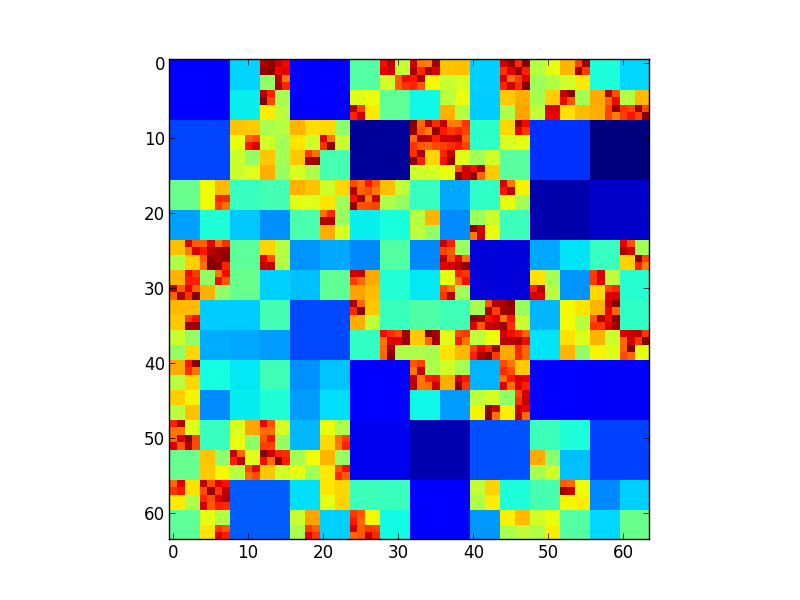
\includegraphics[width=0.75\textwidth]{./images/figure_p13_1.png}
  \caption{Performance comparison across remap methods: compact hash, perfect hash, hierarchical hash, and traditional kD-tree.}
  \label{fig:performance_comparison}
\end{figure}

\section{Discussion}

Our results suggest that hash-based mesh remapping techniques offer a powerful alternative to traditional spatial data structures like kD-trees and quadtrees. The main advantages stem from their simpler control flow, better parallelism, and improved memory efficiency—particularly in heterogeneous environments like multi-core CPUs and GPUs.

In cases with structured or moderately unstructured AMR meshes, perfect hashes offer an efficient and collision-free remap solution. However, their memory footprint can become problematic in sparse mesh configurations. In these situations, compact hashing becomes advantageous by minimizing memory usage, though it introduces minor overhead due to sentinel value handling.

The hierarchical hash further provides a balanced solution for mixed-resolution meshes, especially where varying levels of refinement are present across the domain. This method effectively localizes memory operations and allows more control over spatial granularity.

Comparative tests with brute force methods (which scale as $\mathcal{O}(n^2)$) and tree-based methods (typically $\mathcal{O}(n \log n)$) confirm that hashing strategies consistently achieve better asymptotic and real-world performance. While brute force is often used for result validation due to its simplicity, it is not viable for large-scale simulations. Tree-based methods suffer from traversal overhead and are harder to optimize on parallel hardware due to recursive logic and synchronization issues.

It is worth noting that as meshes become increasingly unstructured or irregular—such as in real-time fluid dynamics or astrophysics simulations—the advantages of hashing become even more pronounced. The decoupling of data through hashing reduces the number of candidate intersections significantly and eliminates many expensive geometric calculations.

Future extensions of this work could explore dynamic hash-based remapping strategies and adaptive hash sizing to further optimize performance based on mesh characteristics and runtime conditions.

\begin{figure}[h]
  \centering
  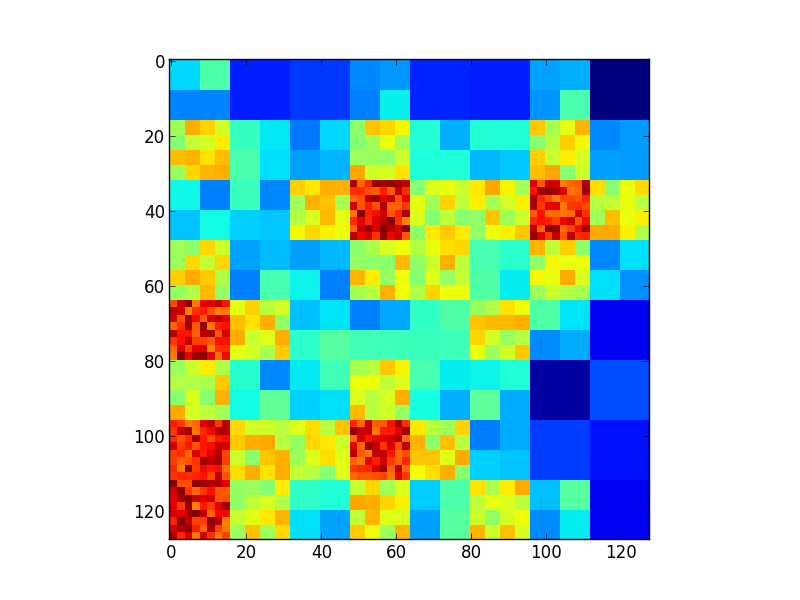
\includegraphics[width=0.75\textwidth]{./images/figure_p13_2.png}
  \caption{Summary visualization of method efficiency and suitability across mesh types.}
  \label{fig:discussion_summary}
\end{figure}

The idea of using attention mechanisms to reduce unnecessary computation draws inspiration from the transformer architecture~\cite{Vaswani2017}.


\bibliographystyle{plain}
\bibliography{references}

\end{document}
